\documentclass[a4paper, 12pt]{article}
\usepackage[utf8]{inputenc}
\usepackage[czech]{babel}
\usepackage[left=2cm, top=3cm, text={17cm, 24cm}]{geometry}
\usepackage{graphicx}
\graphicspath{ {./images/} }
\usepackage{fancyhdr}
\usepackage{enumitem}
\usepackage{tabularx}
\usepackage{url}
\usepackage{xcolor}
\usepackage{listings}
\usepackage[unicode, colorlinks, hypertexnames=false, citecolor=red]{hyperref}
\usepackage{tabto}
\usepackage{placeins}
\hypersetup{colorlinks = true, hypertexnames = false}
\usepackage{pdflscape}

\setlength\parindent{0pt}

\usepackage{fancyvrb}

% redefine \VerbatimInput
\RecustomVerbatimCommand{\VerbatimInput}{VerbatimInput}%
{fontsize=\footnotesize,
 %
 frame=lines,  % top and bottom rule only
 framesep=2em, % separation between frame and text
 rulecolor=\color{gray},
 %
 label=\fbox{\color{black}udpData.txt},
 labelposition=topline,
 %
 %commandchars=\|\(\), % escape character and argument delimiters for
                      % commands within the verbatim
 %commentchar=*        % comment character
}

\lstdefinestyle{BashInputStyle}{
  language=bash,
  basicstyle=\small\sffamily,
  %numbers=left,
  %numberstyle=\scriptsize,
  %numbersep=3pt,
  frame=tb,
  columns=fullflexible,
  backgroundcolor=\color{cyan!5},
  linewidth=0.9\linewidth,
  %xleftmargin=0.1\linewidth
}

\newcommand*{\Package}[1]{\texttt{#1}}

\definecolor{dkgreen}{rgb}{0,0.6,0}
\definecolor{gray}{rgb}{0.5,0.5,0.5}
\definecolor{mauve}{rgb}{0.58,0,0.82}

\lstdefinestyle{CLanguage}{
  language=C,
  aboveskip=3mm,
  belowskip=3mm,
  showstringspaces=false,
  columns=flexible,
  basicstyle={\small\ttfamily},
  numbers=none,
  numberstyle=\tiny\color{gray},
  keywordstyle=\color{blue},
  commentstyle=\color{dkgreen},
  stringstyle=\color{mauve},
  breaklines=true,
  breakatwhitespace=true,
  tabsize=3,
  inputencoding=utf8,
  extendedchars=true,
  literate={á}{{\'a}}1 {ú}{{\'a}}1 {é}{{\'e}}1 {í}{{\'i}}1   {ý}{{\'y}}1 {č}{{\v{c}}}1 {ť}{{\'t}}1 {ľ}{{\'l}}1 
}

\begin{document}

    %Titulni strana
    \begin{titlepage}
        \begin{center}
            
\includegraphics[width=0.87\textwidth]{logo_cz.png}
            \vspace*{6cm}

            \Huge{\textbf{Mikroprocesorové a vestavěné systémy}}
            \vspace{0.5cm}
            
            \LARGE{ESP32: Přístupový terminál}
            \vspace{1cm}
            
            \Large{David Chocholatý (xchoch09)}
            
           \vfill
		   \begin{flushright} 
		   Brno, \today
		   \end{flushright}
        \end{center}
    \end{titlepage}

\pagestyle{fancy}
\lhead{\bfseries ESP32: Přístupový terminál}
\rhead{\bfseries xchoch09}

\newpage
\tableofcontents
\newpage

\section{Úvod}
Cílem projektu bylo navrhnout a implementovat přístupový terminál za použití klávesnice a dvou led diod značících stav \textit{otevřeno} či \textit{zavřeno}. Implementace byla vytvořena s použitím vývojové desky ESP32 v jazyce C.

\section{Zapojení hardware}
Poskytnutý hardware včetně ESP, klávesnice, rezistorů a led diod byl zapojen následovně:


\begin{figure}[!htbp]
    \begin{center}
        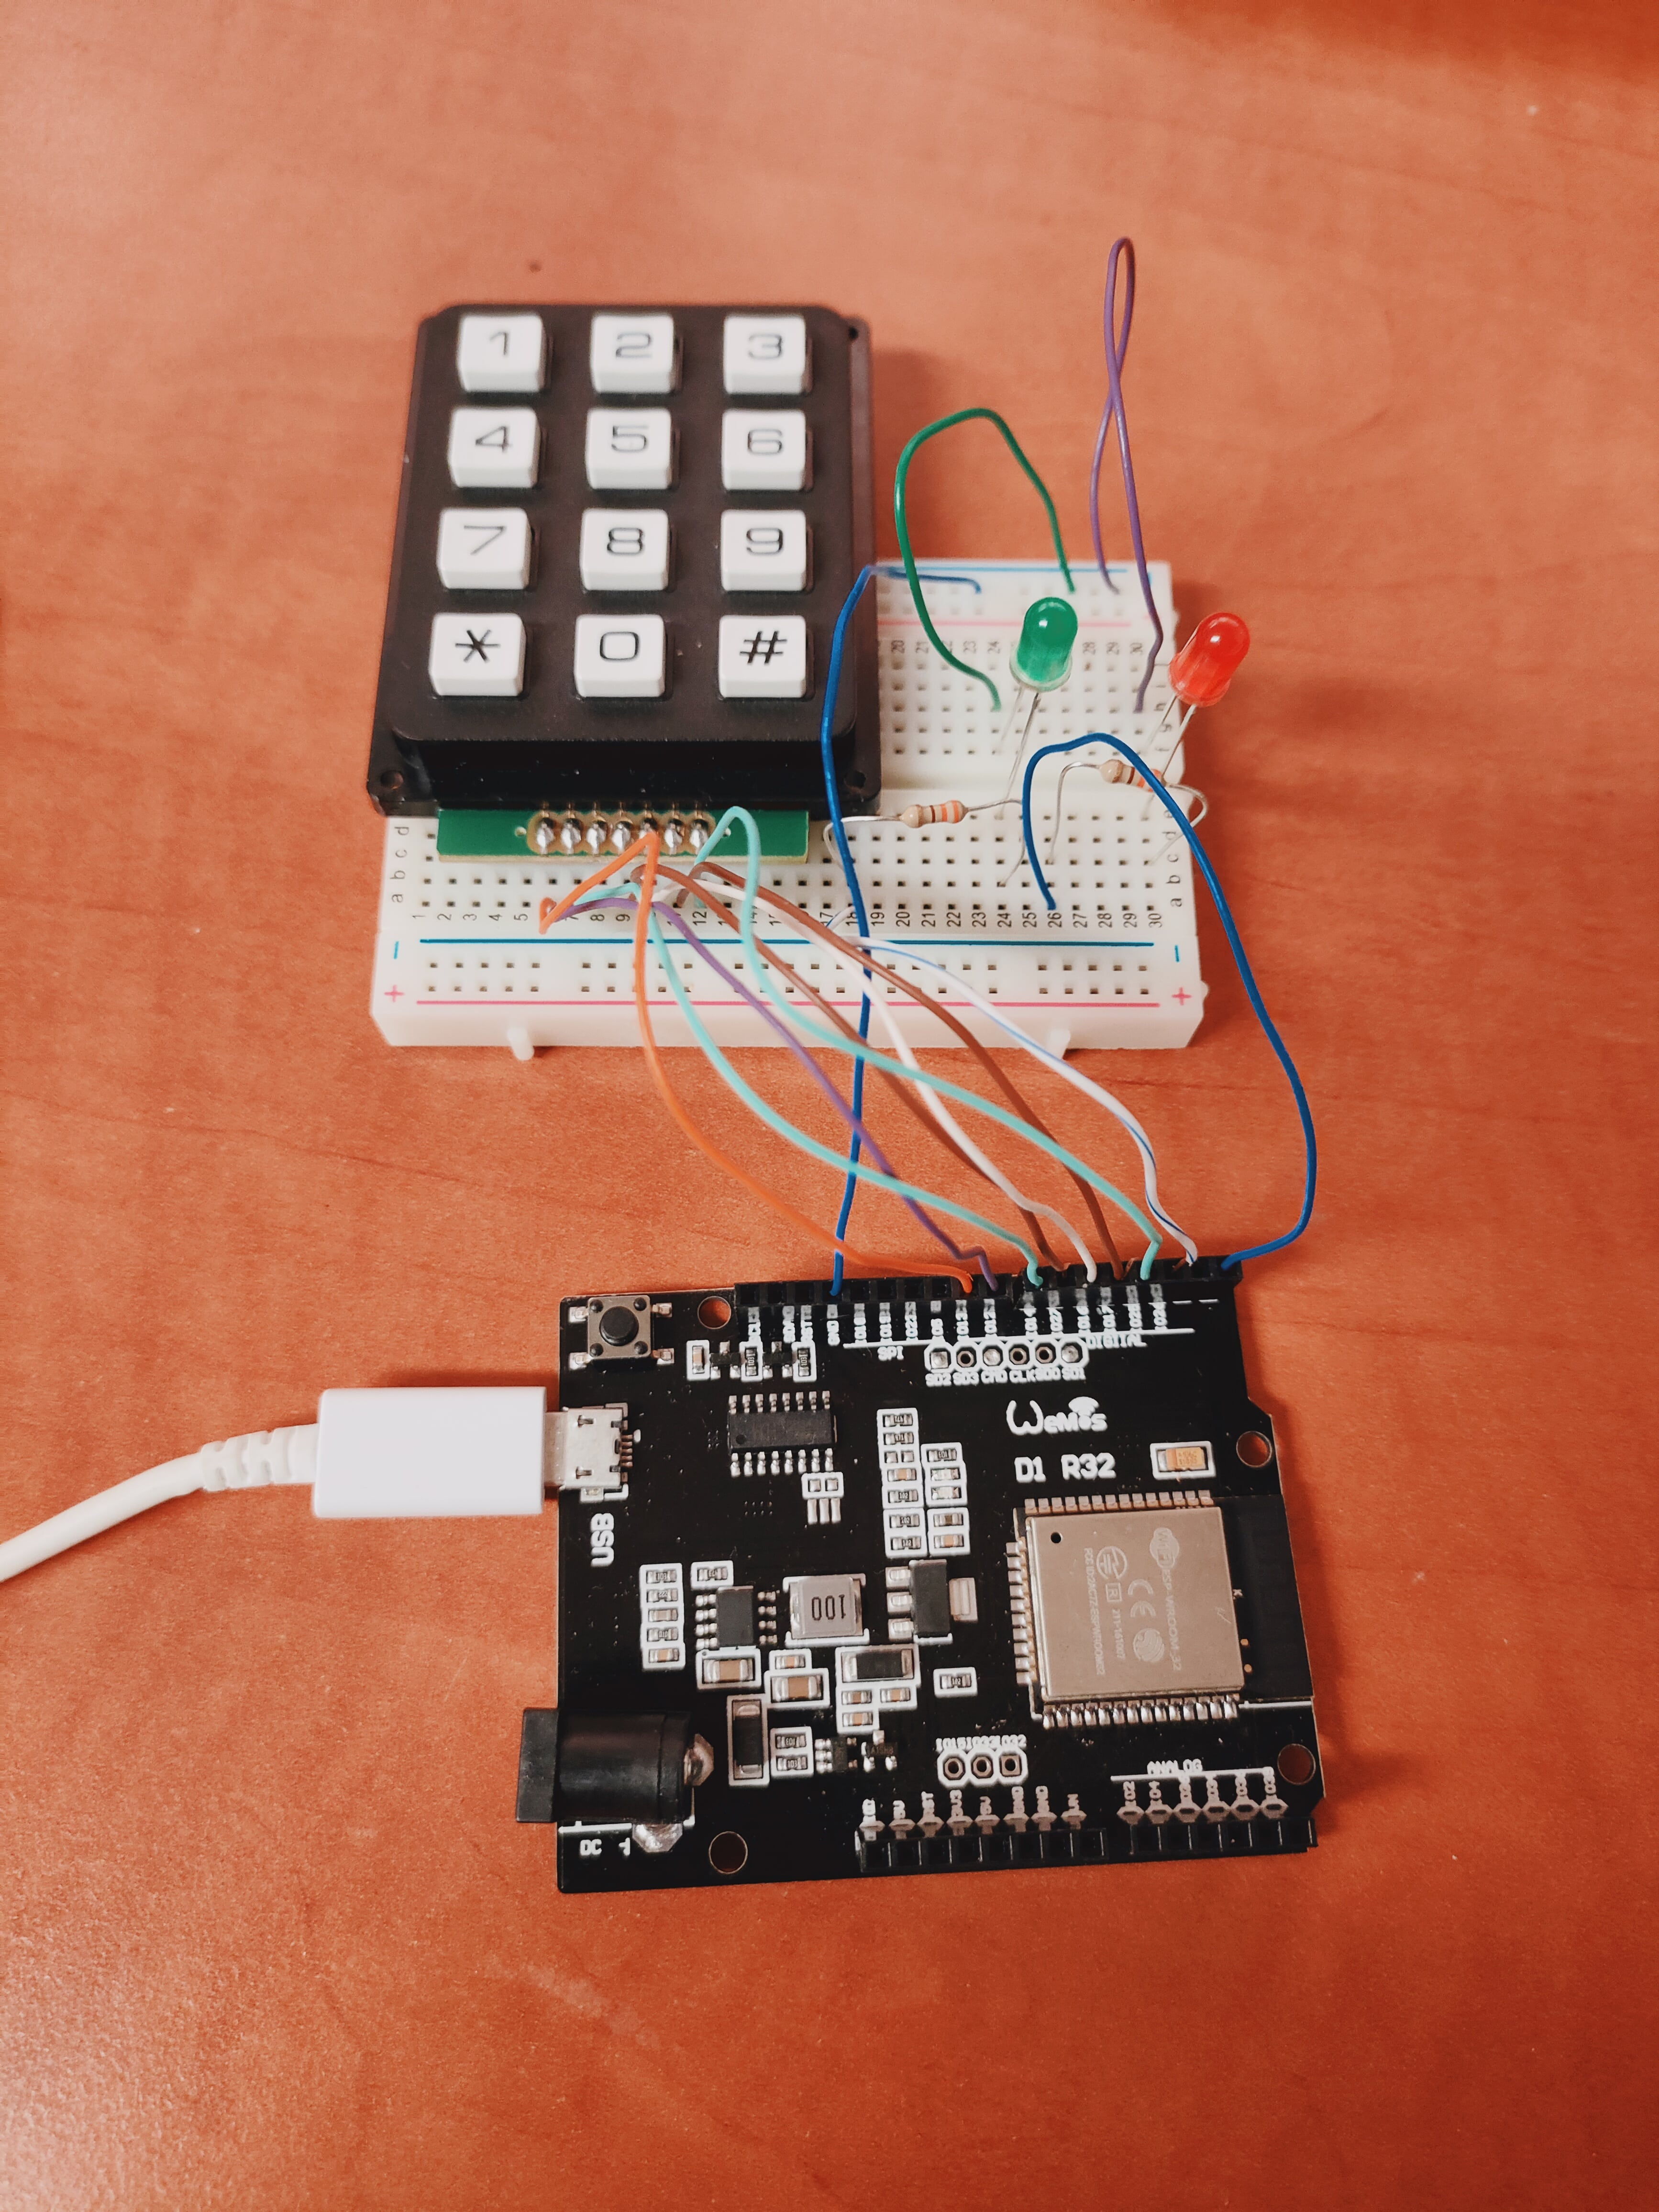
\includegraphics[width=0.7\textwidth]{images/hardware.jpg}
        \caption{Zapojení hardware}
    \end{center}
\end{figure}
\FloatBarrier

\newpage

Zapojení jednotlivých pinů lze nalézt přímo ve zdrojovém souboru \textit{main.c}, kde zapojení pinů pro implementaci specifikuje následující úsek kódu

\begin{lstlisting}[style=CLanguage]
/******************************/
/*         LED DIODES         */
/******************************/

// The pin for the green led.
#define GREEN_LED_PIN GPIO_NUM_26
// The pin for the red led.
#define RED_LED_PIN GPIO_NUM_3

/******************************/
/*        MATRIX KEYPAD       */
/******************************/
// The pin for the first row.
#define MATRIX_KP_ROW_1 GPIO_NUM_12
// The pin for the second row.
#define MATRIX_KP_ROW_2 GPIO_NUM_25
// The pin for the third row.
#define MATRIX_KP_ROW_3 GPIO_NUM_17
// The pin for the fourth row.
#define MATRIX_KP_ROW_4 GPIO_NUM_27
// The pin for the first column.
#define MATRIX_KP_COL_1 GPIO_NUM_14
// The pin for the second column.
#define MATRIX_KP_COL_2 GPIO_NUM_13
// The pin for the third column.
#define MATRIX_KP_COL_3 GPIO_NUM_16
\end{lstlisting}

\vspace{0.25cm}

ze kterého vyplývá zapojení prvků:

\begin{itemize}
\begin{minipage}{0.35\linewidth}   
        \item Zelená led dioda        
        \item Červená led dioda
        \item První řádek klávesnice
        \item Druhý řádek klávesnice
        \item Třetí řádek klávesnice
        \item Čtvrtý řádek klávesnice        
        \item První sloupec klávesnice
        \item Druhý sloupec klávesnice
        \item Třetí sloupec klávesnice        
        %\vspace{0.25cm}
    \end{minipage}
    \begin{minipage}{0.5\linewidth}
        \item[-] GPIO 26
        \item[-] GPIO 3
        \item[-] GPIO 12
        \item[-] GPIO 25
        \item[-] GPIO 17
        \item[-] GPIO 27
        \item[-] GPIO 14
        \item[-] GPIO 13
        \item[-] GPIO 16
    \end{minipage}
\end{itemize}

\newpage

\section{Návod ke spuštění}
Na spuštění implementace přístupového terminálu jsou zapotřebí následující požadavky:

\begin{itemize}
    \item Aplikace \textit{Visual Studio Code} (dále jen \textit{VS Code})\cite{vsCode}.
    \item Nainstalovaný plugin \textit{PlatformIO}\cite{platformio} do aplikace \textit{VS Code}.
\end{itemize}

Po instalaci všech potřebných požadavků lze přejít k připojení vývojové desky ESP32 k počítači přes USB. Dále v nastavení rozšíření \textit{PlatformIO} lze zjistít číslo portu, na kterém je zařízení připojené, a to v nastavení \textit{Devices}.

Po zkontrolování připojení zařízení dále je možné postupovat dvěma způsoby:

\begin{enumerate}[label=(\alph*)]
    \item Přeložení a spuštění již vytvořeného projektu.

        \begin{itemize}
            \item Nejprve bude přiložený projekt otevřen v programu \textit{VS Code}. Dále je nutné, aby konfigurace obsahovala správný port, na kterém je připojená vývojová deska ESP32. To se provádí pomocí příkazu \textit{upload\_port} v souboru \textit{platformio.ini} nacházejícím se v kořenové složce projektu. Ve výchozím nastavení projektu je vývojová deska očekávána na portu \textit{COM4}.
        \end{itemize}
    
    \item Vytvoření nového projektu, manuální konfigurace a nahrazení obsahu souboru \textit{main.c} za vytvořenou implementaci.

        \begin{itemize}
            \item Tento způsob spuštění projektu popisuje počáteční vytvoření projektu s popisem všech konfiguračních kroků. Nejprve tedy bude vytvořen nový projekt pomocí rozšíření \textit{PlatformIO}. Jako vývojová deska bude zvolena deska \textit{Espressif ESP32 Dev Module} a framework \textit{Espressif IoT Development Framework}.

            Jako další krok bude nastaven zvolený port, na kterém je zařízení připojeno také do konfiguračního souboru rozšíření \textit{PlatformIO}. Konkrétněji do souboru \textit{platformio.ini}, nacházejícím se v kořenové složce projektu, bude přidán řádek \textit{upload\_port = COM4} pro očekávání připojení vývojové desky na port \textit{COM4}. V konfiguraci projektu ještě bude nastavena monitorovací rychlost 115200 baudů pomocí následujícího řádku: \textit{monitor\_speed = 115200}.
            
            Nyní lze přejít k poslednímu konfiguračnímu kroku, a to k vypnutí sledování procesoru ve stavu IDLE pomocí Watchdog. Pro použití tohoto projektu lze dané sledování zakázat. To bude provedeno pomocí následujícího nastavení v souboru \textit{sdkconfig.esp32dev}:
            
            \begin{itemize}
                \item[] \textit{CONFIG\_ESP\_TASK\_WDT\_CHECK\_IDLE\_TASK\_CPU0=n}
                \item[] \textit{CONFIG\_ESP\_TASK\_WDT\_CHECK\_IDLE\_TASK\_CPU1=n}
            \end{itemize}
            
            Nyní již byly všechny konfigurační kroky provedeny a lze nahradit obsah souboru \textit{main.c} nacházejícího se ve složce \textit{src/} za vytvořenou implementaci.
        \end{itemize}    
\end{enumerate}

Nyní lze přejít k samotnému překladu a spuštění projektu přístupového terminálu. To lze provést pomocí úlohy \textit{Upload and Monitor} v rozšíření \textit{PlatformIO}.


\section{Implementace}
Pro vytvoření implementace byla především použita oficiální dokumentace k vývojovým deskám ESP\cite{espDoc}. Dále také pro seznámení s novým zařízením byly použity oficiální příklady od společnosti Espressif\cite{espExamples}.

\subsection{Konfigurace GPIO pinů}
Jako první krok algoritmu po spuštění programu jsou neprve nakonfigurovány GPIO piny, a to nejprve pro obsluhu led diod a poté pro obsluhu klávesnice.

\subsubsection*{GPIO pro led diody}
Piny obsluhující led diody jsou nejprve nastaveny do výchozího stavu pomocí funkce \textit{gpio\_reset\_pin()}. Dále jsou piny nakonfigurovány pomocí následujícího úseku kódu:

\begin{lstlisting}[style=CLanguage]
// Initialize the config structure.
gpio_config_t io_conf = {                
    // Set as input mode.
    .mode = GPIO_MODE_OUTPUT,
    // Disable pull-down mode.
    .pull_down_en = GPIO_PULLDOWN_DISABLE,
    // Enable pull-up mode.
    .pull_up_en = GPIO_PULLUP_DISABLE,
    // Disable interrupt.
    .intr_type = GPIO_INTR_DISABLE
};
\end{lstlisting}

GPIO piny jsou tedy nastaveny jako výstupní a oba rezistory (pull down a pull up) jsou zakázány. To stejné platí i pro obsluhu přerušení.
Následně po nastavení konfigurace je přirazena k daným dvěma pinům obsluhující led diody a poté je port přiřazený k červené led diodě nastaven na hodnotu 1. Pin obsluhující zelenou led diodu je nastaven na hodnotu 0. Celý zmíněný úsek algoritmu lze nalézt ve funkci \textit{configure\_leds()}.

\subsubsection*{GPIO pro klávesnici}
Dále jsou nakonfigurovány GPIO piny pro obsluhu klávesnice. Nejprve je vytvořena konfigurace totožná jak pro piny obsluhující řádky klávesnice, tak i pro piny obsluhující sloupce. Následující úsek kódu popisuje zmíněné nastavení:

\begin{lstlisting}[style=CLanguage]
// Initialize the config structure.
gpio_config_t io_conf = {                
    // Set as input mode.
    .mode = GPIO_MODE_INPUT_OUTPUT_OD,
    // Disable pull-down mode.
    .pull_down_en = GPIO_PULLDOWN_DISABLE,
    // Enable pull-up mode.
    .pull_up_en = GPIO_PULLUP_ENABLE
};  
\end{lstlisting}

Nyní konfigurace definuje nastavení módu pinu zároveň povolující vstupní i výstupní mód s povolením módu otevřeného kolektoru (open-drain mode). Dále je z rezistorů povolen pouze pull up rezistor. Pull down rezistor je opět zakázán.

Daná konfigurace je přiřazena nejprve pinům pro obsluhu sloupců klávesnice. Pro tyto piny je zakázána obsluha přerušení pomocí příkazu \textit{io\_conf.intr\_type = GPIO\_INTR\_DISABLE}. Dále je dokončená konfigurace přiřazena všem pinům pro obsluhu sloupců a jejich výstupní hodnota je nastavena na hodnotu 0.

Piny pro obsluhu řádků klávesnice použivají dříve definované nastavení, které bylo použito pro konfiguraci pinů obsluhující sloupce, ovšem nyní je obsluha přerušení povolena, a to pouze při sestupné hraně signálu pomocí příkazu \textit{io\_conf.intr\_type = GPIO\_INTR\_NEGEDGE}. Upravená konfigurace je poté přiřazena všem pinům obsluhující řádky klávesnice a jejich výstupní hodnota je nastavena na hodnotu 1. Popsaný úsek algoritmu lze nalézt ve funkci \textit{configure\_matrix\_keypad()}.

\subsection{Zpracování přerušení}
Po konfiguraci všech GPIO pinů obsluhujících klávesnici je v totožné funkci \textit{configure\_matrix\_keypad()} nastaveno zpracování přerušení zaznamenaných pouze na řádcích klávesnice.

Nejprve je obsluha vytvořena pomocí funkce \textit{xTaskCreate} následujícím příkazem:

\begin{lstlisting}[style=CLanguage]
// Start gpio task.    
xTaskCreate(matrix_kp_row_isr_callback, "matrix_kp_row_isr_callback", 2048, NULL, 5, NULL);
\end{lstlisting}

poté nainstalována služba obsluhy ISR:

\begin{lstlisting}[style=CLanguage]
// Install gpio isr service.
ESP_ERROR_CHECK(gpio_install_isr_service(ESP_INTR_FLAG_DEFAULT));
\end{lstlisting}

a přidán ovladač ISR pouze pro GPIO piny obsluhující řádky klávesnice:

\begin{lstlisting}[style=CLanguage]
// Hook isr handler for specific gpio pin.
ESP_ERROR_CHECK(gpio_isr_handler_add(MATRIX_KP_ROW_1, gpio_isr_handler, (void*) MATRIX_KP_ROW_1));
ESP_ERROR_CHECK(gpio_isr_handler_add(MATRIX_KP_ROW_2, gpio_isr_handler, (void*) MATRIX_KP_ROW_2));
ESP_ERROR_CHECK(gpio_isr_handler_add(MATRIX_KP_ROW_3, gpio_isr_handler, (void*) MATRIX_KP_ROW_3));
ESP_ERROR_CHECK(gpio_isr_handler_add(MATRIX_KP_ROW_4, gpio_isr_handler, (void*) MATRIX_KP_ROW_4));
\end{lstlisting}

Pro obsluhu přerušení je také vytvořena fronta pro zpracování událostí GPIO z ISR pomocí funkce \textit{xQueueCreate()}.

Samotné přerušení obsluhuje funkce \textit{gpio\_isr\_handler()}:

\begin{lstlisting}[style=CLanguage]
/*
 * The gpio isr handler for all matrix rows.
 */
static void IRAM_ATTR gpio_isr_handler(void* arg)
{
    uint32_t gpio_num = (uint32_t) arg;
    xQueueSendFromISR(gpio_evt_queue, &gpio_num, NULL);    
}
\end{lstlisting}

která především vkládá položku do vytvořené fronty pomocí funkce \textit{xQueueSendFromISR()}.

Nyní jsou všechny konfigurační úkony dokončeny včetně popisu zpracování přerušení a lze přejít k části algoritmu zpracovávající detekci stisku tlačítka.

\subsection{Detekce stisku tlačítka}
Detekování a zpracování stisku tlačítka je vytvořeno ve funkci \textit{matrix\_kp\_row\_isr\_callback()}, která byla přiřazena k úlohám již ve funkci \textit{xTaskCreate()}. Úloha je implementována jako nekonečná smyčka pomocí cyklu \textit{for(;;)}. Poté je položka přijmuta z fronty pomocí úseku kódu:

\begin{lstlisting}[style=CLanguage]
if(xQueueReceive(gpio_evt_queue, &io_num, portMAX_DELAY) == pdTRUE) {
...
\end{lstlisting}

Pro otestování hodnoty stisku tlačítka je implementováno čekání pro odeznění zákmitu signálu na začátku stisku tlačítka (anglicky tzv. debounce). Tuto funkcionalitu implementuje stejnojmenná funkce:

\begin{lstlisting}[style=CLanguage]
/*
 * The function for debouncing the matrix keypad button press.
 */
static int debounce(uint32_t io_num)
{
    // Register task to be associated with a watchdog.
    ESP_ERROR_CHECK(esp_task_wdt_add(NULL));

    int previous_level;
    int current_level;

    previous_level = gpio_get_level(io_num);

    for (int i = 0; i < DEBOUNCE_TIME_MS; i++) {
        vTaskDelay(1 / portTICK_PERIOD_MS); // Wait for 1 millisecond.

        current_level = gpio_get_level(io_num);

        if (current_level != previous_level) {            
            i = 0; // Start again.
            previous_level = current_level;
        }

        // Explicitly feed the watchdog.
        ESP_ERROR_CHECK(esp_task_wdt_reset());
    }

    // Unsubscribe the task from the watchdog.
    ESP_ERROR_CHECK(esp_task_wdt_delete(NULL));

    return current_level;
}
\end{lstlisting}

Pro odeznění zákmitu lze zmínit, že je použitý o něco jiný typ algorimu, než pouhé čekání po určitou dobu pro další otestování hodnoty tlačítka, po které se předpokládá, že zákmit odezněl. Implementovaný algoritmus nejprve si zaznamená aktuální hodnotu na daném portu. Poté algoritmus přechází do cyklu, který provádí určitý počet iterací. Jelikož v každé iteraci algoritmus provádí čekání pomocí funkce \textit{vTaskDelay()} po dobu jedné milisekundy, počet iterací určuje celkovou dobu čekání (v implementaci je použita hodnota 10 iterací). Ovšem zmíněná funkce neimplementuje pouhé čekání, ale po uplynutí jedné milisekundy opět testuje hodnotu na daném pinu. Pokud hodnota neodpovídá původní hodnotě, ještě probíhá zmíněný zákmit. Z tohoto důvodu je počet provedených iterací opět vynulován a poslední zaznamenaná hodnota na pinu je nastavena jako aktuální. Na tomto základě tedy počet iterací určuje dobu, po kterou je hodnota na pinu neměnná (čekání po dobu jedné milisekundy, které je provedeno v 10 iteracích, kdy v každé iteraci je získaná hodnota totožná s předchozí). Po odeznění zákmitu lze přejít k hlavní logice samotného zpracování stisku tlačítka.

Nejprve je pro GPIO pin, na kterém bylo detekováno přerušení, nastavena výstupní hodnota z hodnoty 1 na 0. Poté je pro všechny piny obsluhující sloupce klávesnice nastavena výstupní hodnota z hodnoty 0 na 1. Danou logiku provádí následující úsek kódu:

\begin{lstlisting}[style=CLanguage]
// Switch the matrix keypad gpio levels to check in which column
// the pressed pad is.
ESP_ERROR_CHECK(gpio_set_level(io_num, 0));
ESP_ERROR_CHECK(gpio_set_level(MATRIX_KP_COL_1, 1));
ESP_ERROR_CHECK(gpio_set_level(MATRIX_KP_COL_2, 1));
ESP_ERROR_CHECK(gpio_set_level(MATRIX_KP_COL_3, 1));
\end{lstlisting}

Cílem této logiky je po určení řádku klávesnice, na kterém se nachází stisknuté tlačítko, také určit sloupec, ve kterém se tlačítko nachází a tím i definování hodnoty stisknutého tlačítka dle rozložení poskytnuté klávesnice.

Určení sloupce, ve kterém se nachází stisknuté tlačítko se provádí pomocí testování vstupní hodnoty GPIO pinu, který obsluhuje daný sloupec. Například pro první sloupec je daná logika provedena následujícím úsekem kódu:

\begin{lstlisting}[style=CLanguage]
if (gpio_get_level(MATRIX_KP_COL_1) == 0) {  
...
\end{lstlisting}

Poté již implementace využívá konstrukce \textit{switch} pro určení GPIO pinu, který obsluhuje daný řádek, na kterém se nachází stistknuté tlačítko, a na kterém bylo vyvoláno přerušení. Poté po určení správného řádku a sloupce je určena hodnota stisknutého tlačítka.

Jako předposlední krok algoritmus používá testování, zda uživatel nedrží tlačítko stisknuté po delší dobu. Pokud ano, je tato situace ošetřena tak, že pomocí cyklu \textit{while} se provádí čekání, dokud uživatel tlačítko nepustí do výchozí polohy. Danou logiku implementuje následující úsek kódu (například pro první sloupec klávesnice):

\begin{lstlisting}[style=CLanguage]
// Loop here while pressed until the user lets go.
while (gpio_get_level(MATRIX_KP_COL_1) == 0) {
    vTaskDelay(10 / portTICK_PERIOD_MS);
}
...

\end{lstlisting}

Po detekování a zpracování stisku tlačítka již mohou být změněné výstupní hodnoty navráceny na hodnoty původní. Pro GPIO pin obsluhující řádek, na kterém bylo vyvoláno přerušení, bude výstupní hodnota navrácena zpět na hodnotu 1 a výstupní hodnota pro všechny piny obsluhující sloupce klávesnice je navrácena na hodnotu 0. Poté již funkce pouze provádí část algoritmu pro zpracování hesla.

\subsection{Práce s kódem (heslem)}

\subsubsection*{Definice}

Pro práci s kódem (heslem) je definována struktura \textit{password}:

\begin{lstlisting}[style=CLanguage]
/******************************/
/*          PASSWORD          */
/******************************/
typedef struct password {
    char *password_reference;
    char *password_data;
    uint32_t password_length;
    uint32_t password_position;
    bool change_password_auth_state;
    bool change_password_auth_flag;
    bool change_password_write_state;
} password_t;
\end{lstlisting}

Hodnoty jednotlivých proměnných struktury jsou nastaveny pomocí následujícího úseku kódu:

\begin{lstlisting}[style=CLanguage]
/******************************/
/*          PASSWORD          */
/******************************/

// Default configuration for the password handling structure.
#define PASSWORD_DEFAULT_CONFIG() \
{                                 \
    .change_password_auth_state = false, \
    .change_password_auth_flag = false, \
    .change_password_write_state = false, \
    .password_length = 4,         \
    .password_position = 0,       \
    .password_reference = (char[]) {'1', '2', '3', '4', '\0'}, \
    .password_data = (char[]) {'x', 'x', 'x', 'x', '\0'}  \
}
\end{lstlisting}

Délka kódu, neboli hesla, je pevně nastavena na délku 4 znaků. Jako výchozí heslo je nastaveno heslo \textit{1234}. Dále je proměnná obsahující ukazatel na pole, ve kterém budou uloženy znaky zadané uživatelem na klávesnici, inicializována tak, že každý znak je ve výchozím nastavení zastoupen znakem \textit{x}, který není obsažen na poskytnuté klávesnici (výchozí zadané heslo je tedy heslo \textit{xxxx}). Struktura také definuje tři proměnné pro práci s heslem, a to proměnné

\begin{itemize}
    \item \textit{change\_password\_auth\_state}
    \item \textit{change\_password\_auth\_flag}
    \item \textit{change\_password\_write\_state}
\end{itemize}

První proměnná (\textit{change\_password\_auth\_state}) slouží pro nastavení stavu systému, kdy uživatel stiskl tlačítko na klávesnici se znakem \textit{*}. V takovém případě uživatel začíná sekvenci kroků, kdy chce změnit současné heslo za heslo nové. Pokud po zadání znaku \textit{*} zadá správné heslo, při kontrole zadaného hesla implementace nespouští vizuální signalizaci pro zadání správného hesla, ovšem přepíná systém do druhého stavu, a to do stavu kdy je nastaven příznak identifikující správné zadání původního hesla při změně hesla (proměnná \textit{\textit{change\_password\_auth\_flag}}). Poslední proměnná (\textit{change\_password\_write\_state}) slouží pro přepnutí systému do stavu, kdy uživatel chce měnit aktuální heslo za nové, správně zadal původní heslo a po zadání tohoto hesla bylo stisknuto tlačítko se znakem \textit{\#}, za kterým nyní bude následovat heslo nové. Právě tento stav zadávání nového hesla reprezentuje zmíněná proměnná.

\subsubsection*{Zaznamenání znaku kódu (hesla)}
Po detekci a zpracování stisku tlačítka na klávesnici již lze identifikovat hodnotu stisknutého tlačítka. Pro každý znak kromě znaků \textit{*} a \textit{\#} je znak zaznamenán do pole obsahujícího zadané heslo a je aktualizována aktuální pozice ve zmíněném poli. Danou logiku provádí úsek kódu:

\begin{lstlisting}[style=CLanguage]
password.password_data[password.password_position] = value;
password.password_position++;
...
\end{lstlisting}

Obsluha znaků \textit{*} a \textit{\#} při práci s heslem je implementována specificky dle požadovaného chování a zohledňující všechny okrajové případy, které budou dále zmíněny.

\subsubsection*{Ověření správnosti kódu (hesla)}
Ověření správnosti kódu provádí následující úsek kódu:

\begin{lstlisting}[style=CLanguage]
// The length of the entered password is the same as the length
// of the checked password.
if (password.password_position == password.password_length) {
    password.password_position = 0;

    // Check if the user tries to set a new password. 
    if (password.change_password_write_state) {
        // The user entered the new password which should be set
        // as a new one. So, this state is still valid and
        // the new password will be set.
        
        password.change_password_write_state = false;

        // Set the new password
        strcpy(password.password_reference, password.password_data);

        ESP_LOGI(TAG, "password has been successfully changed");

        password_changed_signalization();

    } else {
        // Test if the entered password is correct.
        if (strcmp(password.password_reference, password.password_data) == 0) {
            // The entered password is correct.

            // Check if the user wants to set the new password.
            if (password.change_password_auth_state) {                            
                // Successful password check when changing password.
                password.change_password_auth_state = false;
                password.change_password_auth_flag = true;

                ESP_LOGI(TAG, "successful authentication when changing the password");
            } else {
                // Otherwise, the user just to want to enter.
                ESP_LOGI(TAG, "passwords match");

                access_allowed_signalization();                                
            }
            
        } else {
            // The entered password is incorrect.

            // Check if the user wants to set the new password (auth state).
            if (password.change_password_auth_state) {
                // Delete the auth state.
                password.change_password_auth_state = false;
            }
            
            // The entered password is incorrect.
            ESP_LOGI(TAG, "passwords are different");

            access_denied_signalization();                                                    
        }
    }                                  
}
\end{lstlisting}

Testování správnosti zadaného hesla je porovnáváno pouze v případě, že všechny požadované znaky kódu, neboli hesla, byly zadány a zároveň se systém nenachází ve stavu, kdy bylo zadáno nové heslo, které nyní má být heslem referenčním (heslo je změněno a je spuštěna příslušná vizuální signalizace). V případě zadání všech znaků kódu (hesla) je pozice v zadaném heslu nastavena opět na výchozí hodnotu 0 značící začátek pole obsahujícího zadané heslo. Poté lze přejít k porovnání zadaného hesla a požadovaného hesla pomocí funkce \textit{strcmp()}. Nyní lze odděleně popsat následující dvě situace:

\begin{enumerate}[label=(\alph*)]
    \item Zadané heslo je správné

    \begin{itemize}
        \item Pokud zadané heslo je správné, může se systém nacházet ve dvou stavech. Pokud se systém nachází ve výchozím stavu, je spuštěna příslušná vizuální signalizace značící zadání správného kódu (hesla). Pokud ne, nachází se ve stavu změny hesla, kdy uživatel splnil první část sekvence kroků, a to zadání původního, a v tomto případě správného hesla. Pro tuto situaci je systém přepnut do stavu, kdy je nastaven příznak značící správně zadané heslo.
    \end{itemize}
    
    \item Zadané heslo není správné

    \begin{itemize}
        \item Pokud zadané heslo není správné, je případný stav systému značící zadávání původního hesla při změně hesla vynulován a v každém případě je spuštěna příslušná vizuální signalizace značící nevalidní kód (heslo).
    \end{itemize}
    
\end{enumerate}

\subsection{Implementované okrajové případy}
Implementace podporuje také následující okrajové případy (viz přiložené video).

\begin{itemize}
    \item Zadání nesprávného původního hesla při změně kódu.
    \item Na pozici znaku \textit{\#} při změně hesla se nachází jiný znak.
    \item Nové heslo obsahuje znak \textit{*} nebo \textit{\#}.
    \item Nové heslo je totožné s původním heslem (heslo je nahrazeno heslem totožným).
    \item Ve výchozím stavu znak \textit{\#} slouží pro vymazání již zadané části hesla, pokud již nebylo zadané celé heslo.
\end{itemize}

\subsection{Vizuální signalizace}
Implementace podporuje vizuální signalizaci pro tři následující situace (a jim implementované funkce):

\begin{itemize}
\begin{minipage}{0.45\linewidth}   
        \item \textit{access\_allowed\_signalization()}   
        \vspace{0.5cm}
        \item \textit{access\_denied\_signalization()}
        \vspace{0.5cm}
        \vspace{0.5cm}
        \item \textit{password\_changed\_signalization()}
        %\vspace{0.25cm}
    \end{minipage}
    \begin{minipage}{0.4\linewidth}
        \item[-] signalizace správného hesla (přístup povolen)
        \item[-] signalizace nesprávného hesla (přístup odmítnut) nebo nesprávné práce s klávesnicí
        \item[-] signalizace úspěšné změny hesla
    \end{minipage}
\end{itemize}

\subsection{Watchdog}
Při práci s vývojovou deskou ESP32 byla také nutná práce z tzv. \textit{Watchdog}. Tato část je provedena nejprve v konfiguraci a poté i v samotném kódu. Při konfiguraci je vypnuto sledování procesoru ve stavu IDLE pomocí následujícího nastavení v souboru \textit{sdkconfig.esp32dev}:

\begin{itemize}
    \item[] \textit{CONFIG\_ESP\_TASK\_WDT\_CHECK\_IDLE\_TASK\_CPU0=n}
    \item[] \textit{CONFIG\_ESP\_TASK\_WDT\_CHECK\_IDLE\_TASK\_CPU1=n}
\end{itemize}

Pro záměr tohoto projektu lze tuto kontrolu vypnout a vynechat tuto v jiných případěch vhodnou funkcionalitu.

Dále je pracováno s \textit{Watchdog} i v samotné implementaci. Nejprve je pomocí funkce \textit{esp\_task\_wdt\_init()} inicializován \textit{Task Watchdog Timer (TWDT)}. Při konfiguraci je časový limit nastaven na hodnotu 2 sekundy a je zakázáno vyvolání tzv. paniky (\textit{panic handler}). Poté je na začátku každé funkce (mimo funkcí \textit{gpio\_isr\_handler()} a \textit{matrix\_kp\_row\_isr\_callback()}) registrována úloha k \textit{Watchdog} pomocí příkazu \textit{esp\_task\_wdt\_add(NULL)}, případně v průběhu funkce je \textit{Watchdog} explicitně periodicky informován o validním průběhu práce systému pomocí funkce \textit{esp\_task\_wdt\_reset()}, aby bylo zabráněno vypršení časového limitu. Na konci funkce je každá úloha odregistrována od \textit{Watchdog} pomocí příkazu \textit{esp\_task\_wdt\_delete(NULL)}.

\subsection{Ověření validity řešení}
Po dokončení implementace bylo řešení důkladě testováno jak na jednotlivé případy užití, které zmiňuje oficiální zadání, tak i na případy užití definované autorem, které zadání rozšiřují. Během práce se systémem se systém nedostal do nežádoucího stavu či neprováděl jiné, než požadované úkony. Na základě důkladného otestování a demostrace funkčnosti řešení pomocí videa lze tímto podpořit a konstatovat validitu implementovaného řešení.

\newpage

\section{Autoevaluace}
Na základě vypracování projektu lze provést autoevaluaci pro následující kritéria hodnocení.

\subsection{Přístup (E)}
Přístup k projektu lze hodnotit pozitivně. Projekt byl řešen s dostatečným časovým předstihem. Nejprve autor projektu si pečlivě nastudoval podstatné informace pro práci s vývojovou deskou ESP32 a vyzkoušel pár testovacích a ukázkových oficiálních příkladu pro otestování funkčnosti zařízení a seznámení se s vývojem na dané platformě. Autor při implementaci pracoval i nad rámec oficiálního zadání, implementoval podporu i pro okrajové případy a navrhnul vhodné způsoby signalizace pro jednotlivé situace, které mohou při práci se systémem nastat.

\subsection{Funkčnost (F)}
Implementace projektu splňuje veškerou požadovanou funkcionalitu, kterou, jak již bylo řečeno, rozšiřuje pro ošetření a podporu okrajových případů. Při práci se systémem během testování nenastala situace, kdy by se systém dostal do nepožadovaného stavu či pracoval nesprávně. Na základě testování lze tímto podpořit validitu implementovaného řešení.

\subsection{Kvalita (Q)}
Autor projektu implementoval různé způsoby signalizace pomocí dvou led diod (červené a zelené) nad rámec oficiálního zadání. Tímto byla zvýšení především uživatelská přívětivost systému. Dále byl projekt implementován s důrazem na kvalitu a čistotu zdrojového kódu a veškerá funkcionalita je popsána i přiloženými odpovídajícími komentáři. Již struktura dokumentace napovídá o preciznosti dekompozice projektu na jednotlivé podproblémy a dílčí úkony, které jsou implementovaným algoritmem prováděny.

\subsection{Prezentace (P)}
Po dokončení implementace projektu bylo autorem vytvořeno prezentační komentované video, kde ukazuje i se slovním popisem práci se systémem a jednotlivé implementované a podporované situace.

\subsection{Dokumentace (D)}
Tato dokumentace obsahuje jak úvod do problematiky, tak také definování cíle projektu. Dále je popsáno zapojení poskytnutého hardware a konfigurace projektu nutná pro správné spuštění implementace. Dokumentace je důkladně rozdělena do kapitol dle jednotlivých podproblémů, kde v každé kapitole je problém následně důkladně vysvětlen a popsán. Vytvořená ukázka také obsahuje části kódu ke slovnímu popisu pro lepší názornost řešení. Dokumentace také zmiňuje výčet implementovaných okrajových řešeních nad rámec oficiálního zadání projektu a popisuje ověření validity implementovaného řešení. Na závěr autor projektu provádí finální autoevaluaci.

\bibliographystyle{czechiso}
\renewcommand{\refname}{Použitá literatura}
\bibliography{main}

\end{document}
